\documentclass[../main.tex]{subfiles}
\graphicspath{{\subfix{../images/}}}
\begin{document}

\subsection{Batch Sizes and Learning Rates}

The batch size being used to train the model impacts the amount that is updated on each step. Larger batch sizes means fewer updates. To compensate for the decrease in updates, the learning rates need to be adjusted. Currently, there is only 1 image in every batch. To test the impact of batch size on our data, several quantities of batch sizes should be tested.

\subsubsection{Related Work}

Dominic Masters and Carlo Luschi \cite{DBLP:journals/corr/abs-1804-07612} concluded from their paper that "the best results have been obtained with batch sizes m = 32 or smaller, often as small as m = 2 or m = 4". In this paper, different batch sizes were trialled and they found that there was a general performance increase with reduced batch sizes. This result was obtained with the use of the linear scaling rule which states that an increase in the batch size requires a proportional increase to the learning rate to keep the mean weight update constant during gradient descent. Using the suggestions from the paper, several batch sizes up to 32 are tested. 

\begin{figure}[h!]
  \centering
  \begin{subfigure}[b]{0.3\linewidth}
    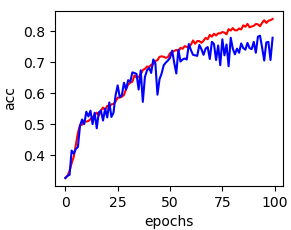
\includegraphics[width=\linewidth]{batch-size-img/bs2.png}
    \caption{Batch Size 2}
  \end{subfigure}
  \begin{subfigure}[b]{0.3\linewidth}
    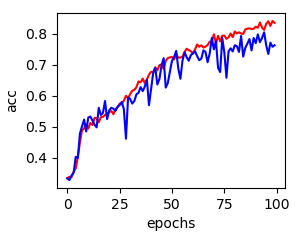
\includegraphics[width=\linewidth]{batch-size-img/bs4.png}
    \caption{Batch Size 4}
  \end{subfigure}
  \begin{subfigure}[b]{0.3\linewidth}
    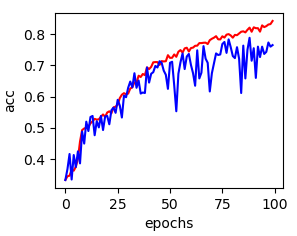
\includegraphics[width=\linewidth]{batch-size-img/bs8.png}
    \caption{Batch Size 8}
  \end{subfigure}
\end{figure}

\begin{figure}[h!]
  \centering
  \begin{subfigure}[b]{0.3\linewidth}
    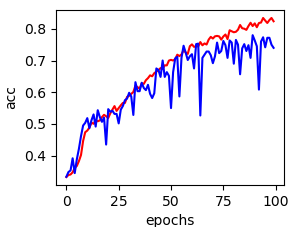
\includegraphics[width=\linewidth]{batch-size-img/bs16.png}
    \caption{Batch Size 16}
  \end{subfigure}
  \begin{subfigure}[b]{0.3\linewidth}
    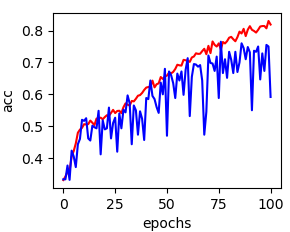
\includegraphics[width=\linewidth]{batch-size-img/bs32.png}
    \caption{Batch Size 32}
  \end{subfigure}
\end{figure}

From these results, it can be seen that the models had about the same highest accuracy of around 75\% or 80\%. This result does not align with the study because the training set of 3000 images is small compared to the training set of CIFAR10 containing 50000 images used in the paper. 

However, when the batch size and learning rate are larger, the accuracy fluctuates much more. This is because the learning rate is too high so too large of updates are occurring. Because of this fluctuation of the accuracy, the confidence we can have in the model is much less so lower batch sizes should be used.

\end{document}